\chapter{Конструкторский раздел}\label{ch:ch2}
\section{Обоснование выбора языка программирования}\label{sec:ch2/sec1}

\subsection{Сравнение языков программирования}\label{sec:ch2/sec1/sub1}
Для разработки {\ProgModule} понадобится сверхвысокоуровневый язык с кросс-платформенной
стандартной библиотекой, который позволит точно и лаконично описать этапы анализа,
а так же имеющий высокую скорость исполнения, для анализа больших объемов исходного кода и
исполняемых файлов.

\begin{table}
    {\small
        \setlength{\tabcolsep}{2pt}
        \caption{\label{table:languages-comparsion}
               Сравнительная таблица языков программирования}
        \begin{longtable}{*{5}{| c}|}
            \hline
            \diagbox[width=8cm]{Свойства}{Язык программирования} &
                \makecell{Nim \autocite{nim}} &
                \makecell{Python \autocite{python}} &
                \makecell{Perl \autocite{perl}} &
                \makecell{C/C++} \\
            \hline
                \makecell{Сверхвысокоуровневость} & 
                \greencell{Да} & 
                \greencell{Да} &
                \greencell{Да} &
                \redcell{Нет} \\
            \hline
                \makecell{Компилируется в\\машинный код} & 
                \greencell{Да} & 
                \redcell{Нет} &
                \redcell{Нет} &
                \greencell{Да} \\
            \hline
                \makecell{Количество функции в\\стандартной библиотеке} & 
                5585 & 
                638 &
                1338 &
                1224 \\
            \hline
                \makecell{Портируемость} & 
                \greencell{Есть} & 
                \greencell{Есть} &
                \greencell{Есть} &
                \yellowcell{\makecell{Есть,\\но неудобная}}\\
            \hline
                \makecell{Встроенная\\генерация документации} & 
                \greencell{Есть} & 
                \greencell{Есть} &
                \greencell{Есть} &
                \redcell{Нет}\\
            \hline
                \makecell{Статическая типизация} & 
                \greencell{Есть} & 
                \redcell{Нет} &
                \redcell{Нет} &
                \greencell{Есть}\\
            \hline
                \makecell{Автоматическое\\управление памятью} & 
                \greencell{Есть} & 
                \greencell{Есть} &
                \greencell{Есть} &
                \greencell{Есть} \\
            \hline
                \makecell{Обобщенное программирование} & 
                \greencell{Есть} & 
                \greencell{Есть} &
                \greencell{Есть} &
                \greencell{Есть} \\
            \hline
                \makecell{Опыт использования} & 
                \greencell{Есть} & 
                \greencell{Есть} &
                \redcell{Нет} &
                \greencell{Есть} \\
            \hline
        \end{longtable}
    }
\end{table}

Рассмотрим подробно каждый из представленных в таблице языков.

\subsubsection{C++}\label{sec:ch2/sec1/sub1/sub1}
Мультипарадигменный высокоуровневый язык программирования,
разработанный в 1983 году Бьёрном Страуструпом. Является практически
полным надмножеством языка C. Статически типизирован.\\
Отличается высокой производительностью и неплохой гибкостью при написании кода.
К минусам языка можно отнести сложность освоения и перегруженность 
<<наследием>> 80-х годов прошлого века, а так же низкую скорость компиляции,
по сравнению с предшественником -- C.\\
Портируемость языка на различные платформы обеспечивается пере- или
кросс-компиляцией исходного кода под нужную платформу.


\subsubsection{Python}\label{sec:ch2/sec1/sub1/sub2}
Мультипарадигменный сверхвысокоуровневый язык программирования,
разработанный в 1991 году Гвидо Ван Россумом.
Является интерпретируемым языком, имеет слабую динамическую типизацию,
что позволяет легко писать обобщенный код и использовать мета-программирование,
но так же ведет к трудноулавливаемым ошибкам. Негативное влияние можно сгладить
с помощью указания типов при объявлении перемнных и аргументов функций, а так же 
программы, проверяющей эти типы -- линтера. Например pylint \autocite{pylint} или
pyflakes \autocite{pyflakes}.\\
Благодаря своей популярности, python так же портирован на большое количество платформ.
Большим плюсом языка является его обширная стандартная библиотека, позволяющая легко
писать комплексные приложения, не прибегая к установке дополнительных библиотек --
такие программы, как и сам python, следуют философии <<в комплекте с батарейками>>
(<<batteries included>> \autocite{batteries-included}), суть которой заключается в 
самодостаточности программ. Помимо этого вместе с python поставляется менеджер
пакетов pip \autocite{pip}, позволяющий удобно устанавливать требуемые библиотечные модули вместе
с зависимостями.\\
К минусам языка можно отнести медлительность эталонного интерпретатора языка -- cpython \autocite{cpython}.
Код, исполняемый им, в определенных задачах медленнее кода на C в сотни раз. Не смотря на то, что
есть более быстрые интерпретаторы: PyPy \autocite{pypy}, Jython \autocite{jython}, Iron Python \autocite{iron-python},
они не смогут достичь скорости исполнения программ, компилируемых в машинный код.\\
На данный момент существует две, между собой несовместимые, версии языка: 
python 2, поддержка которого закончилась \DTMdate{2020-01-01} и python 3.

\subsubsection{Perl}\label{sec:ch2/sec1/sub1/sub2}
Мультипарадигменный сверхвысокоуровневый 
язык программирования, разработанный в 1987 году Ларри Уоллом.
Является интерпретируемым языком, имеет слабую динамическую типизацию.\\
Полное название языка -- <<Practical Extraction and Report Language>> 
(<<Практический Язык для Извлечения Данных и Составления Отчётов>>), отражает его суть:
в языке реализованы обширные возможности для работы с текстом, в синтаксис интегрированы 
регулярные выражения, как и в языках, которые оказали на него наибольшее влияние --
AWK \autocite{awk} и sed \autocite{sed}. Но это же и я является его слабой частью, так как
Perl скорее предназначен для однострочных команд в терминале, как AWK и
sed.
        
\subsubsection{Nim}\label{sec:ch2/sec1/sub1/sub3}
Мультипарадигменный сверхвысокоуровневый 
язык программирования, разработанный в 2004 году Андреасом Румпфом.
Является компилируемым языком, имеет строгую статическую типизацию.\\
Заметно, что на синтаксис языка повлиял Python, что сделало его
выразительным и понятным. Язык использует промежуточную компиляцию, которая несколько
замедляет процесс компиляции программ, но позволяет запускать nim-программы на различных
платформах. На данный момент поддерживается компиляция в JavaScript \autocite{javascript}
и оптимизированный C-код с несколькими моделями управления памятью:\\
\begin{itemize}
    \item Сборщики мусора, основанные на:
        \begin{enumerate}
            \item подсчете ссылок;
            \item подсчете ссылок с оптимизацией move-семантикой \autocite{nim-gc-move}:
            \item boehm \autocite{boehm-gc};
            \item go \autocite{go-gc};
        \end{enumerate}
    \item ручном освобождении памяти;
    \item модель, в которой вся выделенная память высвобождается только по завершению программы;
        (не рекомендуется к использованию)
\end{itemize}
Компиляции Nim в C означает не только высокую скорость работы, но и прозрачный программный интерфейс при взаимодействии с
C библиотеками. Это значит, что можно писать Nim-код, взаимодействующий с С библиотекой так же, как
если бы это была Nim-библиотека, в отличие от, например, Python.\\
Так же вместе с компилятором языка поставляется пакетный менеджер nimble \autocite{nimble} и генератор
документации из комментариев, написанных на reStructuredText \autocite{restructuredtext}.

\subsubsection{Вывод}\label{sec:ch2/sec1/sub1/sub4}
Из всего вышесказанного следует, что для {\ProgModule} лучше всего подойдет язык Nim
благодаря его скорости, выразительности и портируемости на различные платформы.
Кроме того, для подготовки динамического анализа программы будут использованы утилиты, умеющие разбирать
заголовки исполняемого файла, а именно objdump и readelf. Форматирование входных данных для данных утилит
будет осуществляться с помощью Bash-скриптов.

\subsection{Обоснование выбора среды разработки}\label{sec:ch2/sec1/sub2}

\subsection{Сравнение сред разработки}\label{sec:ch2/sec1/sub1}

Для разработки на Nim существует несколько IDE и огромное количество
текстовых редакторов, часть которых рассмотрим ниже:

\begin{table}[!htbp]
    {\small
        \setlength{\tabcolsep}{2pt}
        \caption{\label{table:ide-comparsion}
               Сравнительная таблица IDE и редакторов кода}
        \begin{longtable}{*{6}{| c}|}
            \hline
            \diagbox[width=8cm]{Свойства}{IDE/Редактор} &
                \makecell{Aporia \autocite{aporia-ide}} &
                \makecell{Atom \autocite{atom-ide}} &
                \makecell{Sublime\\Text \autocite{sublime-ide}} &
                \makecell{Visual\\Studio\\Code \autocite{vs-code-ide}} &
                \makecell{Vim \autocite{vim-ide}} \\
            \hline
                \makecell{Поддержка плагинов} & 
                \redcell{Нет} &
                \greencell{Да} & 
                \greencell{Да} &
                \greencell{Да} &
                \greencell{Да} \\
            \hline
                \makecell{Требователен к ресурсам} & 
                \greencell{Нет} & 
                \redcell{Да} & 
                \greencell{Нет} & 
                \redcell{Да} & 
                \greencell{Нет} \\ 
            \hline
                \makecell{Имеет продвинутую систему\\редактирования текста} & 
                \redcell{Нет} &
                \redcell{Нет} &
                \redcell{Нет} &
                \redcell{Нет} &
                \greencell{Да} \\
            \hline
                \makecell{Кросс-платформенность} & 
                \greencell{Есть} & 
                \greencell{Есть} &
                \greencell{Есть} &
                \greencell{Есть} &
                \greencell{Есть} \\
            \hline
                \makecell{Может работать\\без GUI} & 
                \redcell{Нет} &
                \redcell{Нет} &
                \redcell{Нет} &
                \redcell{Нет} &
                \greencell{Да} \\
            \hline
                \makecell{Восстановление после сбоев} & 
                \redcell{Нет} & 
                \greencell{Есть} &
                \greencell{Есть} &
                \greencell{Есть} &
                \greencell{Есть} \\
            \hline
                \makecell{Возможность выделять\\ключевые слова с помощью\\регулярных выражений} & 
                \redcell{Нет} & 
                \greencell{Есть} &
                \greencell{Есть} &
                \greencell{Есть} &
                \greencell{Есть} \\
            \hline
                \makecell{Опыт использования} & 
                \redcell{Нет} &
                \redcell{Нет} &
                \greencell{Есть} &
                \greencell{Есть} &
                \greencell{Есть} \\
            \hline
        \end{longtable}
    }
\end{table}

Рассмотрим подробно каждый из представленных в таблице редакторов.

\subsubsection{Aporia}\label{sec:ch2/sec1/sub2/sub1}
Простая IDE, написанная на nim, с использованием GTK2.
В настоящее время не поддерживается, так как большая часть Nim-программистов
перешла на Visual Studio Code.

\subsubsection{Atom}\label{sec:ch2/sec1/sub2/sub2}
Редактор от GitHub Inc., написан с использованием Electron \autocite{electron} -- фреймворка
для разработки кросс-платформенных приложений с помощью HTML, JavaScript и CSS. Из-за архитектурных
и технологических решений, все программы, написанные на данном фреймворке, будут очень требовательны
к ресурсам.

\subsubsection{Sublime Text}\label{sec:ch2/sec1/sub2/sub3}
Проприетарный текстовый редактор, возможности которого могут быть расширены
с помощью плагинов на python.

\subsubsection{Visual Studio Code}\label{sec:ch2/sec1/sub2/sub4}
Редактор от Microsoft. Так же, как и Atom, написан с использованием Electron.
Имеет встроенный <<магазин>> плагинов.

\subsubsection{Vim}\label{sec:ch2/sec1/sub2/sub5}
Текстовый редактор с открытым исходным кодом и большими возможностями к
быстрому редактированию текстов. Является наследником редактора vi, который, в свою
очередь, создавался с оглядкой на редактор ed. Управление делится на
режим ввода и режим команд, благодаря чему есть возможность управлять 
редактором только с помощью клавиатуры, что, при должном умении, повышает скорость
не только из-за отсутствия необходимости в использовании компьютерной мыши, но и
более коротким сочетаниям  <<горячих клавиш>>. Легко поддается модифицированию с помощью плагинов.
Есть под множество платформ.


\subsubsection{Вывод}\label{sec:ch2/sec1/sub1/sub4}
Из всего вышесказанного и личного опыта следует, 
что для разработки {\ProgModule} лучше всего подойдет текстовый редактор Vim,
так как он поддерживает добавление плагинов, не требователен к ресурсам и позволяет
очень быстро редактировать текст. В качестве расширения его функциональности использованы
плагины:
\begin{enumerate}
    \item NERDTree \autocite{nerdtree} -- улучшает просмотр каталогов;
    \item Tabular \autocite{tabular} -- позволяет быстро выравнивать текст
        для улучшения читаемости.
    \item vim-polyglot \autocite{vim-polyglot} -- подсветка синтаксиса большого
        числа языков
    \item undotree \autocite{undotree} -- просмотр истории изменений в виде дерева
    \item rainbow \autocite{rainbow} -- подсветка вложенных скобок разными цветами,
        для улучшения читаемости
\end{enumerate}


\begin{figure}[!htbp]
    \centerfloat{
        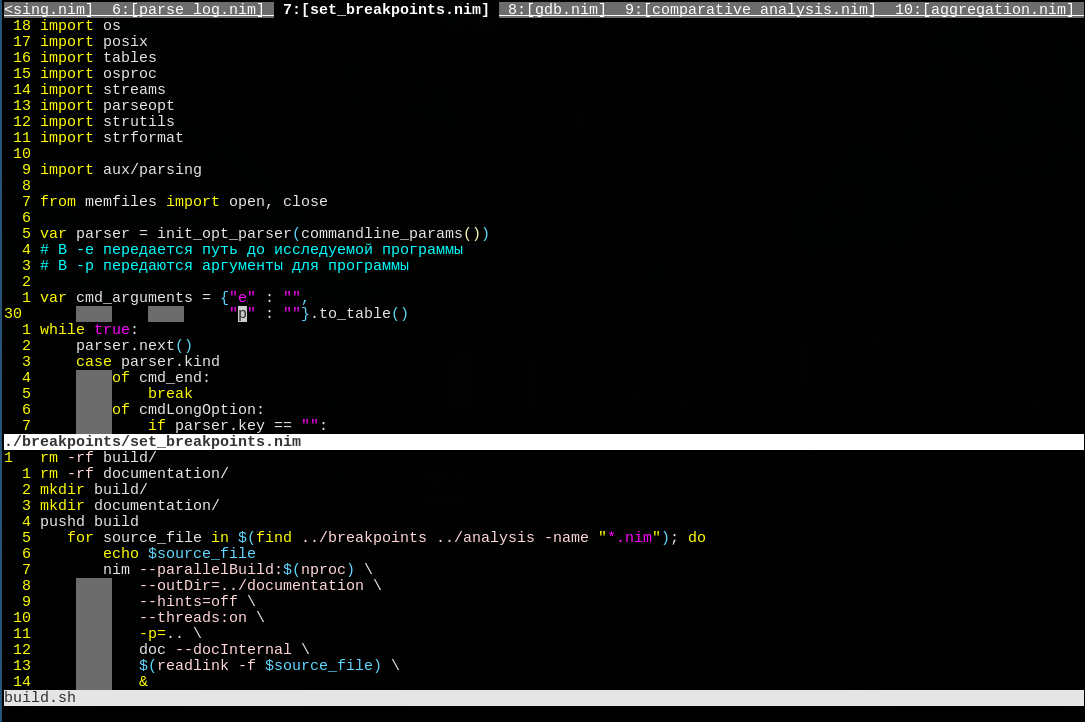
\includegraphics[width=\linewidth]{images/Vim.png}
    }
    \caption{Интерфейс Vim {\ProgModule}\label{fig:vim-tui}}
\end{figure}

\section{Архитектура {\ProgModule}}\label{sec:ch2/sec4}
Архитектура программного обеспечения это система, объединяющая внутрение
компоненты, их связи между собой и с окружением, а так же принципы,
использующиеся при проектировании и эволюции программы \autocite{software-architecture}.

При проектировании {\ProgModule} была выбрана UNIX-философия \autocite{unix-philosophy},
заключающаяся в следующих основопологающих принципах:
\begin{itemize}
    \item создавать маленькие программы;
    \item программы делают одно дело, но делают его хорошо;
    \item хранить данные в текстовом, читаемом для людей формате;
\end{itemize}

Поэтому было принято решение разрабатывать под каждую подзадачу проведения сертификации ПО
самостоятельную программу, которая была бы маленькой и хорошо бы справлялась со своим назначением.

\subsection{Организация передачи информации между компонентами {\ProgModule}}\label{sec:ch2/sec4/sub1}
Передача информации между компонентами {\ProgModule} осуществляется посредством
сериализации внутренних структур конкретного модуля в формате JSON.
JSON удобен тем, что является простым для чтения как человеком, так и компьютером,
что позволяет оператору анализировать так же и промежуточные результаты работы, для
вынесения вердикта.

\subsubsection{Виды сериализуемых данных}\label{sec:ch2/sec4/sub1/sub1}
В {\ProgModule} сериализуются данные после прохождения этапа:
\begin{itemize}
    \item статического анализа исходных кодов;
    \item динамического анализа сертифицируемой программы;
\end{itemize}

\begin{figure}[!htbp]
    \centerfloat{
        % !TEX encoding = UTF-8 Unicode
% Úτƒ-8 encoded
% http://www.linux.org.ru/forum/general/10357036
\tikzset{
    line/.style={draw, -latex'},
    every join/.style={line},
    u/.style={anchor=south},
    r/.style={anchor=west},
    fxd/.style={text width = 6em},
    it/.style={font={\small\itshape}},
    bf/.style={font={\small\bfseries}},
}
\tikzstyle{base} =
    [
        draw,
        on chain,
        on grid,
        align=center,
        minimum height=4ex,
        minimum width = 10ex,
        node distance = 6mm and 60mm,
        text badly centered,
    ]
\tikzstyle{coord} =
    [
        coordinate,
        on chain,
        on grid
    ]
\tikzstyle{cloud} =
    [
        base,
        ellipse,
        node distance = 3cm,
        minimum height = 2em,
        text width=2cm
    ]
\tikzstyle{decision} =
    [
        base,
        diamond,
        aspect=2,
        node distance = 2cm,
        inner sep = 0pt
    ]
\tikzstyle{block} =
    [
        rectangle,
        base,
        rounded corners,
        minimum height = 2em
    ]
\tikzstyle{print_block} =
    [
        base,
        tape,
        tape bend top=none,
    ]
\tikzstyle{io} =
    [
        base,
        trapezium,
        trapezium left angle = 70,
        trapezium right angle = 110,
    ]
\tikzstyle{prompt} =
    [
        base,
        trapezium,
        trapezium left angle = 90,
        trapezium right angle = 80,
        shape border rotate = 90
    ]
\tikzstyle{disk file} =
    [
        base,
        cylinder,
        aspect=0.2,
    ]
\tikzstyle{process} =
    [
        rectangle,
        base,
    ]
\makeatletter
\pgfkeys{/pgf/.cd,
    subrtshape w/.initial=2mm,
    cycleshape w/.initial=2mm
}
\pgfdeclareshape{parallelshape}{
    \inheritsavedanchors[from=rectangle]
    \inheritanchorborder[from=rectangle]
    \inheritanchor[from=rectangle]{north}
    \inheritanchor[from=rectangle]{center}
    \inheritanchor[from=rectangle]{west}
    \inheritanchor[from=rectangle]{east}
    \inheritanchor[from=rectangle]{mid}
    \inheritanchor[from=rectangle]{base}
    \inheritanchor[from=rectangle]{south}
    \backgroundpath{
        \southwest \pgf@xa=\pgf@x \pgf@ya=\pgf@y
        \northeast \pgf@xb=\pgf@x \pgf@yb=\pgf@y
        \def\ppd@offset{\pgfpoint{\pgfutil@tempdima}{0ex}}
        \def\ppd@offsetm{\pgfpoint{-\pgfutil@tempdima}{0ex}}
        \pgfpathmoveto{\pgfqpoint{\pgf@xa}{\pgf@ya}}
            \pgfpathlineto{\pgfqpoint{\pgf@xb}{\pgf@ya}}
        \pgfpathclose
        \pgfpathmoveto{\pgfqpoint{\pgf@xb}{\pgf@yb}}
            \pgfpathlineto{\pgfqpoint{\pgf@xa}{\pgf@yb}}
        \pgfpathclose
    }
}
\pgfdeclareshape{subrtshape}{
    \inheritsavedanchors[from=rectangle]
    \inheritanchorborder[from=rectangle]
    \inheritanchor[from=rectangle]{north}
    \inheritanchor[from=rectangle]{center}
    \inheritanchor[from=rectangle]{west}
    \inheritanchor[from=rectangle]{east}
    \inheritanchor[from=rectangle]{mid}
    \inheritanchor[from=rectangle]{base}
    \inheritanchor[from=rectangle]{south}
    \backgroundpath{
        \southwest \pgf@xa=\pgf@x \pgf@ya=\pgf@y
        \northeast \pgf@xb=\pgf@x \pgf@yb=\pgf@y
        \pgfmathsetlength\pgfutil@tempdima{\pgfkeysvalueof{/pgf/subrtshape w}}
        \def\ppd@offset{\pgfpoint{\pgfutil@tempdima}{0ex}}
        \def\ppd@offsetm{\pgfpoint{-\pgfutil@tempdima}{0ex}}
        \pgfpathmoveto{\pgfqpoint{\pgf@xa}{\pgf@ya}}
        \pgfpathlineto{\pgfqpoint{\pgf@xb}{\pgf@ya}}
        \pgfpathlineto{\pgfqpoint{\pgf@xb}{\pgf@yb}}
        \pgfpathlineto{\pgfqpoint{\pgf@xa}{\pgf@yb}}
        \pgfpathclose
        \pgfpathmoveto{\pgfpointadd{\pgfpoint{\pgf@xa}{\pgf@yb}}{\ppd@offsetm}}
        \pgfpathlineto{\pgfpointadd{\pgfpoint{\pgf@xa}{\pgf@ya}}{\ppd@offsetm}}
        \pgfpathlineto{\pgfpointadd{\pgfpoint{\pgf@xb}{\pgf@ya}}{\ppd@offset}}
        \pgfpathlineto{\pgfpointadd{\pgfpoint{\pgf@xb}{\pgf@yb}}{\ppd@offset}}
        \pgfpathclose
    }
}
\pgfdeclareshape{cyclebegshape}{
    \inheritsavedanchors[from=rectangle]
    \inheritanchorborder[from=rectangle]
    \inheritanchor[from=rectangle]{north}
    \inheritanchor[from=rectangle]{center}
    \inheritanchor[from=rectangle]{west}
    \inheritanchor[from=rectangle]{east}
    \inheritanchor[from=rectangle]{mid}
    \inheritanchor[from=rectangle]{base}
    \inheritanchor[from=rectangle]{south}
    \backgroundpath{
        \southwest \pgf@xa=\pgf@x \pgf@ya=\pgf@y
        \northeast \pgf@xb=\pgf@x \pgf@yb=\pgf@y
        \pgfmathsetlength\pgfutil@tempdima{\pgfkeysvalueof{/pgf/cycleshape w}}
        \pgfpathmoveto{\pgfqpoint{\pgf@xa}{\pgf@ya}}
\pgfpathlineto{\pgfpointadd{\pgfpoint{\pgf@xa}{\pgf@yb}}{\pgfpoint{0ex}{-\pgfutil@tempdima}}}
\pgfpathlineto{\pgfpointadd{\pgfpoint{\pgf@xa}{\pgf@yb}}{\pgfpoint{\pgfutil@tempdima}{0ex}}}
\pgfpathlineto{\pgfpointadd{\pgfpoint{\pgf@xb}{\pgf@yb}}{\pgfpoint{-\pgfutil@tempdima}{0ex}}}
\pgfpathlineto{\pgfpointadd{\pgfpoint{\pgf@xb}{\pgf@yb}}{\pgfpoint{0ex}{-\pgfutil@tempdima}}}
\pgfpathlineto{\pgfqpoint{\pgf@xb}{\pgf@ya}}
        \pgfpathclose
    }
}
\pgfdeclareshape{cycleendshape}{
    \inheritsavedanchors[from=rectangle]
    \inheritanchorborder[from=rectangle]
    \inheritanchor[from=rectangle]{north}
    \inheritanchor[from=rectangle]{center}
    \inheritanchor[from=rectangle]{west}
    \inheritanchor[from=rectangle]{east}
    \inheritanchor[from=rectangle]{mid}
    \inheritanchor[from=rectangle]{base}
    \inheritanchor[from=rectangle]{south}
    \backgroundpath{
        \southwest \pgf@xa=\pgf@x \pgf@ya=\pgf@y
        \northeast \pgf@xb=\pgf@x \pgf@yb=\pgf@y
        \pgfmathsetlength\pgfutil@tempdima{\pgfkeysvalueof{/pgf/cycleshape w}}
        \pgfpathmoveto{\pgfqpoint{\pgf@xb}{\pgf@yb}}
\pgfpathlineto{\pgfpointadd{\pgfpoint{\pgf@xb}{\pgf@ya}}{\pgfpoint{0ex}{\pgfutil@tempdima}}}
\pgfpathlineto{\pgfpointadd{\pgfpoint{\pgf@xb}{\pgf@ya}}{\pgfpoint{-\pgfutil@tempdima}{0ex}}}
\pgfpathlineto{\pgfpointadd{\pgfpoint{\pgf@xa}{\pgf@ya}}{\pgfpoint{\pgfutil@tempdima}{0ex}}}
\pgfpathlineto{\pgfpointadd{\pgfpoint{\pgf@xa}{\pgf@ya}}{\pgfpoint{0ex}{\pgfutil@tempdima}}}
\pgfpathlineto{\pgfqpoint{\pgf@xa}{\pgf@yb}}
        \pgfpathclose
    }
}
\makeatother
\tikzstyle{subroutine} =
    [
        base,
        subrtshape,
    ]
\tikzstyle{cyclebegin} =
    [
        base,
        cyclebegshape,
    ]
\tikzstyle{cycleend} =
    [
        base,
        cycleendshape,
    ]
\tikzstyle{connector} =
    [
        base,
        circle,
    ]

\tikzstyle{parallel} =
    [
        base,
        parallelshape,
    ]

\newcommand{\BreakpointInfo}{
\begin{tabular}{*{2}{| l}|}
BreakpointInfo     & Информация о точке останова\\
\hline
    address        &  адрес, на котором находится точка останова\\
    call\_address   &  адрес, по которому будет совершен вызов\\
    scope\_address  &  адрес функции, внутри которой происходит вызов\\
    registers      &  информация о регистрах процессора в момент останова\\
    instructions   &  восемь инструкций, следующих после команды вызова \\
    backtrace      &  стек вызовов\\
    stack          &  hex-dump стека программы\\
\end{tabular}
}
\newcommand{\SegmentInfo}{
\begin{tabular}{*{2}{| l}|}
SegmentInfo            & Информация о сегментах программы\\
\hline
    name               &  название сегмента\\
    occupied\_mem\_begin &  адрес памяти, с которого начинается сегмент\\
    occupied\_mem\_end   &  адрес памяти, которым заканчивается сегмент\\
\end{tabular}
}

\newcommand{\FunctionInfo}{
\begin{tabular}{*{2}{| l}|}
FunctionInfo & Информация об определенных функциях\\
\hline
    name     &  название функции\\
    address  &  адрес \\
\end{tabular}
}

\newcommand{\ProcessStartInfo}{
\begin{tabular}{*{2}{| l}|}
ProcessStartInfo & Информация о запуске исследуемой программы\\
\hline
    cmdline      &  переданные аргументы\\
    cwd          &  текущая рабочая директория\\
    exe          &  путь к исполняемому файлу\\
\end{tabular}
}

\newcommand{\ProcessSegmentsInfo}{
\begin{tabular}{*{2}{| l}|}
ProcessSegmentsInfo & Информация о всех сегментах программы\\
\hline
    entrypoint      & точка входа в программу\\
    segments        & список информации о сегментах\\
\end{tabular}
}
\newcommand{\Process}{
\begin{tabular}{*{2}{| l}|}
Process              & Информация о исследуемой программе\\
\hline
    pid              &  PID процесса\\
    start\_info       &  информация о запуске программы\\
    segments\_info    &  информация о сегментах программы\\
    breakpoints\_info &  список информации о точках останова\\
    functions\_info   &  список информации об определенных функциях\\
\end{tabular}
}

\begin{tikzpicture}[%
    start chain=going below,    % General flow is top-to-bottom
    node distance=6mm and 30mm, % Global setup of box spacing
    ] 
        \node [process] (breakpointinfo)                                          {\small \BreakpointInfo};
        \node [process] (segmentinfo)        [below = 5cm of breakpointinfo]      {\small \SegmentInfo};
        \node [process] (functioninfo)       [below = 3cm of segmentinfo]         {\small \FunctionInfo};
        \node [process] (processstartinfo)   [below = 3cm of functioninfo]        {\small \ProcessStartInfo};
        \node [process] (processsegmentsinfo)[below = 3cm of processstartinfo]    {\small \ProcessSegmentsInfo};
        \node [process] (process)            [below = 4cm of processsegmentsinfo] {\small \Process};

        \draw [line] (process) -- +(-9,-0) |- (breakpointinfo);
        \draw [line] (process) -- +(-9,-0) |- (segmentinfo);
        \draw [line] (process) -- +(-9,-0) |- (functioninfo);
        \draw [line] (process) -- +(-9,-0) |- (processstartinfo);
        \draw [line] (process) -- +(-9,-0) |- (processsegmentsinfo);

\end{tikzpicture}

    }
    \caption{Сохраняемые структуры динамического анализа \label{fig:dynamic-json}}
\end{figure}

Структура данных помогает иерархически организовать доступ к собранной, во время
динамического анализа, информации.

\texttt{BreakpointInfo} содержит данные с расставленных точек останова, получаемые 
непосредственно во время выполнения машинных инструкций программы, а значит важно
в них получить максимальное количество информации текущем мгновенном состоянии программы.
В структуре содержится:
\begin{itemize}
    \item адреса:
            \begin{itemize}
                \item \texttt{call} инструкции, на которой находится точка останова
                \item по которому собирается сделать вызов \texttt{call} инструкция
                \item функции, в котором находится данная \texttt{call} инструкция
            \end{itemize}
            Которые необходимы для последующего сравнительного анализа;
        \item регистры, в которых могут содержаться передаваемые параметры (fastcall convention \autocite{fastcall});
        \item следующие за \texttt{call} 8 инструкций, в которых может содержаться код, обрабатывающий
            возвращенное значение;
        \item стек вызовов, позволяет посмотреть ветку исполнения исследуемой программы
\end{itemize}

Информация о сегментах в \texttt{SegmentInfo} позволяет определить, к какому сегменту относится
вызываемая, или текущая функция. Например, это может быть сегмент динамически загружаемой библиотеки.

\texttt{FunctionInfo} содержит информацию, которую предоставляет GDB при загрузке программы:
список известных функций и их адреса. Полезно для анализа

\texttt{ProcessStartInfo} сохраняет параметры запуска, \texttt{ProcessSegmentsInfo} -- 
агрегирует информацию по всем сегментам программы.

Структура \texttt{Process} же агрегирует в себе всё вышеперечисленное 

\begin{figure}[!htbp]
    \centerfloat{
        % !TEX encoding = UTF-8 Unicode
% Úτƒ-8 encoded
% http://www.linux.org.ru/forum/general/10357036
\tikzset{
    line/.style={draw, -latex'},
    every join/.style={line},
    u/.style={anchor=south},
    r/.style={anchor=west},
    fxd/.style={text width = 6em},
    it/.style={font={\small\itshape}},
    bf/.style={font={\small\bfseries}},
}
\tikzstyle{base} =
    [
        draw,
        on chain,
        on grid,
        align=center,
        minimum height=4ex,
        minimum width = 10ex,
        node distance = 6mm and 60mm,
        text badly centered,
    ]
\tikzstyle{coord} =
    [
        coordinate,
        on chain,
        on grid
    ]
\tikzstyle{cloud} =
    [
        base,
        ellipse,
        node distance = 3cm,
        minimum height = 2em,
        text width=2cm
    ]
\tikzstyle{decision} =
    [
        base,
        diamond,
        aspect=2,
        node distance = 2cm,
        inner sep = 0pt
    ]
\tikzstyle{block} =
    [
        rectangle,
        base,
        rounded corners,
        minimum height = 2em
    ]
\tikzstyle{print_block} =
    [
        base,
        tape,
        tape bend top=none,
    ]
\tikzstyle{io} =
    [
        base,
        trapezium,
        trapezium left angle = 70,
        trapezium right angle = 110,
    ]
\tikzstyle{prompt} =
    [
        base,
        trapezium,
        trapezium left angle = 90,
        trapezium right angle = 80,
        shape border rotate = 90
    ]
\tikzstyle{disk file} =
    [
        base,
        cylinder,
        aspect=0.2,
    ]
\tikzstyle{process} =
    [
        rectangle,
        base,
    ]
\makeatletter
\pgfkeys{/pgf/.cd,
    subrtshape w/.initial=2mm,
    cycleshape w/.initial=2mm
}
\pgfdeclareshape{parallelshape}{
    \inheritsavedanchors[from=rectangle]
    \inheritanchorborder[from=rectangle]
    \inheritanchor[from=rectangle]{north}
    \inheritanchor[from=rectangle]{center}
    \inheritanchor[from=rectangle]{west}
    \inheritanchor[from=rectangle]{east}
    \inheritanchor[from=rectangle]{mid}
    \inheritanchor[from=rectangle]{base}
    \inheritanchor[from=rectangle]{south}
    \backgroundpath{
        \southwest \pgf@xa=\pgf@x \pgf@ya=\pgf@y
        \northeast \pgf@xb=\pgf@x \pgf@yb=\pgf@y
        \def\ppd@offset{\pgfpoint{\pgfutil@tempdima}{0ex}}
        \def\ppd@offsetm{\pgfpoint{-\pgfutil@tempdima}{0ex}}
        \pgfpathmoveto{\pgfqpoint{\pgf@xa}{\pgf@ya}}
            \pgfpathlineto{\pgfqpoint{\pgf@xb}{\pgf@ya}}
        \pgfpathclose
        \pgfpathmoveto{\pgfqpoint{\pgf@xb}{\pgf@yb}}
            \pgfpathlineto{\pgfqpoint{\pgf@xa}{\pgf@yb}}
        \pgfpathclose
    }
}
\pgfdeclareshape{subrtshape}{
    \inheritsavedanchors[from=rectangle]
    \inheritanchorborder[from=rectangle]
    \inheritanchor[from=rectangle]{north}
    \inheritanchor[from=rectangle]{center}
    \inheritanchor[from=rectangle]{west}
    \inheritanchor[from=rectangle]{east}
    \inheritanchor[from=rectangle]{mid}
    \inheritanchor[from=rectangle]{base}
    \inheritanchor[from=rectangle]{south}
    \backgroundpath{
        \southwest \pgf@xa=\pgf@x \pgf@ya=\pgf@y
        \northeast \pgf@xb=\pgf@x \pgf@yb=\pgf@y
        \pgfmathsetlength\pgfutil@tempdima{\pgfkeysvalueof{/pgf/subrtshape w}}
        \def\ppd@offset{\pgfpoint{\pgfutil@tempdima}{0ex}}
        \def\ppd@offsetm{\pgfpoint{-\pgfutil@tempdima}{0ex}}
        \pgfpathmoveto{\pgfqpoint{\pgf@xa}{\pgf@ya}}
        \pgfpathlineto{\pgfqpoint{\pgf@xb}{\pgf@ya}}
        \pgfpathlineto{\pgfqpoint{\pgf@xb}{\pgf@yb}}
        \pgfpathlineto{\pgfqpoint{\pgf@xa}{\pgf@yb}}
        \pgfpathclose
        \pgfpathmoveto{\pgfpointadd{\pgfpoint{\pgf@xa}{\pgf@yb}}{\ppd@offsetm}}
        \pgfpathlineto{\pgfpointadd{\pgfpoint{\pgf@xa}{\pgf@ya}}{\ppd@offsetm}}
        \pgfpathlineto{\pgfpointadd{\pgfpoint{\pgf@xb}{\pgf@ya}}{\ppd@offset}}
        \pgfpathlineto{\pgfpointadd{\pgfpoint{\pgf@xb}{\pgf@yb}}{\ppd@offset}}
        \pgfpathclose
    }
}
\pgfdeclareshape{cyclebegshape}{
    \inheritsavedanchors[from=rectangle]
    \inheritanchorborder[from=rectangle]
    \inheritanchor[from=rectangle]{north}
    \inheritanchor[from=rectangle]{center}
    \inheritanchor[from=rectangle]{west}
    \inheritanchor[from=rectangle]{east}
    \inheritanchor[from=rectangle]{mid}
    \inheritanchor[from=rectangle]{base}
    \inheritanchor[from=rectangle]{south}
    \backgroundpath{
        \southwest \pgf@xa=\pgf@x \pgf@ya=\pgf@y
        \northeast \pgf@xb=\pgf@x \pgf@yb=\pgf@y
        \pgfmathsetlength\pgfutil@tempdima{\pgfkeysvalueof{/pgf/cycleshape w}}
        \pgfpathmoveto{\pgfqpoint{\pgf@xa}{\pgf@ya}}
\pgfpathlineto{\pgfpointadd{\pgfpoint{\pgf@xa}{\pgf@yb}}{\pgfpoint{0ex}{-\pgfutil@tempdima}}}
\pgfpathlineto{\pgfpointadd{\pgfpoint{\pgf@xa}{\pgf@yb}}{\pgfpoint{\pgfutil@tempdima}{0ex}}}
\pgfpathlineto{\pgfpointadd{\pgfpoint{\pgf@xb}{\pgf@yb}}{\pgfpoint{-\pgfutil@tempdima}{0ex}}}
\pgfpathlineto{\pgfpointadd{\pgfpoint{\pgf@xb}{\pgf@yb}}{\pgfpoint{0ex}{-\pgfutil@tempdima}}}
\pgfpathlineto{\pgfqpoint{\pgf@xb}{\pgf@ya}}
        \pgfpathclose
    }
}
\pgfdeclareshape{cycleendshape}{
    \inheritsavedanchors[from=rectangle]
    \inheritanchorborder[from=rectangle]
    \inheritanchor[from=rectangle]{north}
    \inheritanchor[from=rectangle]{center}
    \inheritanchor[from=rectangle]{west}
    \inheritanchor[from=rectangle]{east}
    \inheritanchor[from=rectangle]{mid}
    \inheritanchor[from=rectangle]{base}
    \inheritanchor[from=rectangle]{south}
    \backgroundpath{
        \southwest \pgf@xa=\pgf@x \pgf@ya=\pgf@y
        \northeast \pgf@xb=\pgf@x \pgf@yb=\pgf@y
        \pgfmathsetlength\pgfutil@tempdima{\pgfkeysvalueof{/pgf/cycleshape w}}
        \pgfpathmoveto{\pgfqpoint{\pgf@xb}{\pgf@yb}}
\pgfpathlineto{\pgfpointadd{\pgfpoint{\pgf@xb}{\pgf@ya}}{\pgfpoint{0ex}{\pgfutil@tempdima}}}
\pgfpathlineto{\pgfpointadd{\pgfpoint{\pgf@xb}{\pgf@ya}}{\pgfpoint{-\pgfutil@tempdima}{0ex}}}
\pgfpathlineto{\pgfpointadd{\pgfpoint{\pgf@xa}{\pgf@ya}}{\pgfpoint{\pgfutil@tempdima}{0ex}}}
\pgfpathlineto{\pgfpointadd{\pgfpoint{\pgf@xa}{\pgf@ya}}{\pgfpoint{0ex}{\pgfutil@tempdima}}}
\pgfpathlineto{\pgfqpoint{\pgf@xa}{\pgf@yb}}
        \pgfpathclose
    }
}
\makeatother
\tikzstyle{subroutine} =
    [
        base,
        subrtshape,
    ]
\tikzstyle{cyclebegin} =
    [
        base,
        cyclebegshape,
    ]
\tikzstyle{cycleend} =
    [
        base,
        cycleendshape,
    ]
\tikzstyle{connector} =
    [
        base,
        circle,
    ]

\tikzstyle{parallel} =
    [
        base,
        parallelshape,
    ]

\newcommand{\UnitInfo}{
\begin{tabular}{*{2}{| l}|}
UnitInfo & Информация об одном файле исходного кода \\
\hline
    arguments           & список аргументов компиляции \\
    directory           & папка с файлом исходного кода \\
    file                & имя файла \\
\end{tabular}
}
\newcommand{\BuildInfo}{
\begin{tabular}{*{2}{| l}|}
BuildInfo  & Информация о сборке программы \\
\hline
        units\_info          & список файлов исходного кода \\
\end{tabular}
}

\newcommand{\FunctionInfo}{
\begin{tabular}{*{2}{| l}|}
    CflowConstruct & Описание функции в статическом анализе \\
\hline
        name         & имя функции \\
        nesting      & уровень вложенности \\
        signature    & сигнатура функции \\
        path         & путь до файла, в котором используется функция \\
        line         & номер строки \\
        recursive    & рекурсивность функции \\
        text\_offset & отступ в сегменте .text \\
\end{tabular}
}

\begin{tikzpicture}[%
    start chain=going below,    % General flow is top-to-bottom
    node distance=6mm and 30mm, % Global setup of box spacing
    ] 
        \node [process] (unitinfo)                                {\small \UnitInfo};
        \node [process] (buildinfo)    [below = 4cm of unitinfo]  {\small \BuildInfo};
        \node [process] (functioninfo) [below = 4cm of buildinfo] {\small \FunctionInfo};


\end{tikzpicture}

    }
    \caption{Сохраняемые структуры статического анализа \label{fig:static-json}}
\end{figure}


\subsection{Cхема данных}\label{sec:ch2/sec4/sub2}

\begin{figure}[!htbp]
    \centerfloat{
        % !TEX encoding = UTF-8 Unicode
% Úτƒ-8 encoded
% http://www.linux.org.ru/forum/general/10357036
\tikzset{
    line/.style={draw, -latex'},
    every join/.style={line},
    u/.style={anchor=south},
    r/.style={anchor=west},
    fxd/.style={text width = 6em},
    it/.style={font={\small\itshape}},
    bf/.style={font={\small\bfseries}}

}
\tikzstyle{base} =
    [
        draw,
        on chain,
        on grid,
        align=center,
        minimum height=4ex,
        minimum width = 10ex,
        node distance = 6mm and 60mm,
        text badly centered,
        text width=5cm
    ]
\tikzstyle{coord} =
    [
        coordinate,
        on chain,
        on grid
    ]
\tikzstyle{cloud} =
    [
        base,
        ellipse,
        node distance = 3cm,
        minimum height = 2em
    ]
\tikzstyle{decision} =
    [
        base,
        diamond,
        aspect=2,
        node distance = 2cm,
        inner sep = 0pt
    ]
\tikzstyle{block} =
    [
        rectangle,
        base,
        rounded corners,
        minimum height = 2em
    ]
\tikzstyle{print_block} =
    [
        base,
        tape,
        tape bend top=none,
    ]
\tikzstyle{io} =
    [
        base,
        trapezium,
        trapezium left angle = 70,
        trapezium right angle = 110,
    ]
\tikzstyle{prompt} =
    [
        base,
        trapezium,
        trapezium left angle = 90,
        trapezium right angle = 80,
        shape border rotate = 90
    ]
\tikzstyle{disk file} =
    [
        base,
        cylinder,
        aspect=0.2,
    ]
\tikzstyle{process} =
    [
        rectangle,
        base,
    ]
\makeatletter
\pgfkeys{/pgf/.cd,
    subrtshape w/.initial=2mm,
    cycleshape w/.initial=2mm
}
\pgfdeclareshape{subrtshape}{
    \inheritsavedanchors[from=rectangle]
    \inheritanchorborder[from=rectangle]
    \inheritanchor[from=rectangle]{north}
    \inheritanchor[from=rectangle]{center}
    \inheritanchor[from=rectangle]{west}
    \inheritanchor[from=rectangle]{east}
    \inheritanchor[from=rectangle]{mid}
    \inheritanchor[from=rectangle]{base}
    \inheritanchor[from=rectangle]{south}
    \backgroundpath{
        \southwest \pgf@xa=\pgf@x \pgf@ya=\pgf@y
        \northeast \pgf@xb=\pgf@x \pgf@yb=\pgf@y
        \pgfmathsetlength\pgfutil@tempdima{\pgfkeysvalueof{/pgf/subrtshape w}}
        \def\ppd@offset{\pgfpoint{\pgfutil@tempdima}{0ex}}
        \def\ppd@offsetm{\pgfpoint{-\pgfutil@tempdima}{0ex}}
        \pgfpathmoveto{\pgfqpoint{\pgf@xa}{\pgf@ya}}
        \pgfpathlineto{\pgfqpoint{\pgf@xb}{\pgf@ya}}
        \pgfpathlineto{\pgfqpoint{\pgf@xb}{\pgf@yb}}
        \pgfpathlineto{\pgfqpoint{\pgf@xa}{\pgf@yb}}
        \pgfpathclose
        \pgfpathmoveto{\pgfpointadd{\pgfpoint{\pgf@xa}{\pgf@yb}}{\ppd@offsetm}}
        \pgfpathlineto{\pgfpointadd{\pgfpoint{\pgf@xa}{\pgf@ya}}{\ppd@offsetm}}
        \pgfpathlineto{\pgfpointadd{\pgfpoint{\pgf@xb}{\pgf@ya}}{\ppd@offset}}
        \pgfpathlineto{\pgfpointadd{\pgfpoint{\pgf@xb}{\pgf@yb}}{\ppd@offset}}
        \pgfpathclose
    }
}
\pgfdeclareshape{cyclebegshape}{
    \inheritsavedanchors[from=rectangle]
    \inheritanchorborder[from=rectangle]
    \inheritanchor[from=rectangle]{north}
    \inheritanchor[from=rectangle]{center}
    \inheritanchor[from=rectangle]{west}
    \inheritanchor[from=rectangle]{east}
    \inheritanchor[from=rectangle]{mid}
    \inheritanchor[from=rectangle]{base}
    \inheritanchor[from=rectangle]{south}
    \backgroundpath{
        \southwest \pgf@xa=\pgf@x \pgf@ya=\pgf@y
        \northeast \pgf@xb=\pgf@x \pgf@yb=\pgf@y
        \pgfmathsetlength\pgfutil@tempdima{\pgfkeysvalueof{/pgf/cycleshape w}}
        \pgfpathmoveto{\pgfqpoint{\pgf@xa}{\pgf@ya}}
\pgfpathlineto{\pgfpointadd{\pgfpoint{\pgf@xa}{\pgf@yb}}{\pgfpoint{0ex}{-\pgfutil@tempdima}}}
\pgfpathlineto{\pgfpointadd{\pgfpoint{\pgf@xa}{\pgf@yb}}{\pgfpoint{\pgfutil@tempdima}{0ex}}}
\pgfpathlineto{\pgfpointadd{\pgfpoint{\pgf@xb}{\pgf@yb}}{\pgfpoint{-\pgfutil@tempdima}{0ex}}}
\pgfpathlineto{\pgfpointadd{\pgfpoint{\pgf@xb}{\pgf@yb}}{\pgfpoint{0ex}{-\pgfutil@tempdima}}}
\pgfpathlineto{\pgfqpoint{\pgf@xb}{\pgf@ya}}
        \pgfpathclose
    }
}
\pgfdeclareshape{cycleendshape}{
    \inheritsavedanchors[from=rectangle]
    \inheritanchorborder[from=rectangle]
    \inheritanchor[from=rectangle]{north}
    \inheritanchor[from=rectangle]{center}
    \inheritanchor[from=rectangle]{west}
    \inheritanchor[from=rectangle]{east}
    \inheritanchor[from=rectangle]{mid}
    \inheritanchor[from=rectangle]{base}
    \inheritanchor[from=rectangle]{south}
    \backgroundpath{
        \southwest \pgf@xa=\pgf@x \pgf@ya=\pgf@y
        \northeast \pgf@xb=\pgf@x \pgf@yb=\pgf@y
        \pgfmathsetlength\pgfutil@tempdima{\pgfkeysvalueof{/pgf/cycleshape w}}
        \pgfpathmoveto{\pgfqpoint{\pgf@xb}{\pgf@yb}}
\pgfpathlineto{\pgfpointadd{\pgfpoint{\pgf@xb}{\pgf@ya}}{\pgfpoint{0ex}{\pgfutil@tempdima}}}
\pgfpathlineto{\pgfpointadd{\pgfpoint{\pgf@xb}{\pgf@ya}}{\pgfpoint{-\pgfutil@tempdima}{0ex}}}
\pgfpathlineto{\pgfpointadd{\pgfpoint{\pgf@xa}{\pgf@ya}}{\pgfpoint{\pgfutil@tempdima}{0ex}}}
\pgfpathlineto{\pgfpointadd{\pgfpoint{\pgf@xa}{\pgf@ya}}{\pgfpoint{0ex}{\pgfutil@tempdima}}}
\pgfpathlineto{\pgfqpoint{\pgf@xa}{\pgf@yb}}
        \pgfpathclose
    }
}
\makeatother
\tikzstyle{subroutine} =
    [
        base,
        subrtshape,
    ]
\tikzstyle{cyclebegin} =
    [
        base,
        cyclebegshape,
    ]
\tikzstyle{cycleend} =
    [
        base,
        cycleendshape,
    ]
\tikzstyle{connector} =
    [
        base,
        circle,
    ]
\begin{tikzpicture}[%
    start chain=going below,    % General flow is top-to-bottom
    node distance=6mm and 30mm, % Global setup of box spacing
    scale=0.7, 
    every node/.style={scale=0.72}
    ] 
        \node [prompt   ] (makefile)        [left  = 2cm ]                      {\small Путь до папки с Makefile};
        \node [process  ] (builder)         [below = 2cm of makefile]           {\small Сборщик};
        \node [prompt   ] (executable)      [right = 10cm of makefile]          {\small Путь до исполняемого файла};
        \node [process  ] (breakpointer)                                        {\small Модуль бинарного анализа};
        \node [disk file] (modified exe)    [below right = 3cm of breakpointer] {\small Модифицированный исполняемый файл};
        \node [disk file] (build log)       [below right = 3cm of builder]      {\small Файл с информацией о сборке};
        \node [process  ] (static analyzer) [below = 3cm of build log]          {\small Модуль статического анализа};
        \node [disk file] (call map)        [below left = 3cm of builder]       {\small Файл с информацией о линковке};
        \node [disk file] (gdb script)      [below left = 3cm of breakpointer]  {\small Скрипт для GDB};
        \node [process  ] (gdb manager)     [below = 4cm of breakpointer]       {\small Модуль управления отладчиком};
        \node [disk file] (dyn result)      [below = 2cm of gdb manager]        {\small Результаты динамического анализа};
        \node [process  ] (dyn parser)      [below = 2cm of dyn result]         {\small Модуль преобразования результатов динамического анализа};
        \node [disk file] (dyn json)        [below = 2cm of dyn parser]         {\small Преобразованные результаты динамического анализа};
        \node [disk file] (stat result)     [below = 2cm of static analyzer]    {\small Результаты статического анализа};
        \node [process  ] (stat parser)     [below = 2cm of stat result]        {\small Модуль преобразования результатов статического анализа};
        \node [disk file] (stat json)       [below = 2cm of stat parser]        {\small Преобразованные результаты статического анализа};
        \node [process  ] (aggregator)      [below = 2cm of stat json]          {\small Модуль агрегирования результатов линковки и статического анализа};
        \node [disk file] (aggregator file) [below = 2cm of aggregator]         {\small Агрегированные результаты линковки и статического анализа};
        \node [process  ] (comparer)                                            {\small Модуль сравнительного анализа};
        \node [disk file] (summary)                                             {\small Результаты сравнительного анализа};

        \draw [line] (makefile)        -- (builder);
        \draw [line] (builder)         -| (call map);
        \draw [line] (builder)         -| (build log);

        \draw [line] (executable)      -- (breakpointer);
        \draw [line] (breakpointer)    -| (modified exe);
        \draw [line] (breakpointer)    -| (gdb script);

        \draw [line] (modified exe)    |- (gdb manager);
        \draw [line] (gdb script)      |- (gdb manager);
        \draw [line] (gdb manager)     -- (dyn result);
        \draw [line] (dyn result)      -- (dyn parser);
        \draw [line] (dyn parser)      -- (dyn json);


        \draw [line] (build log)       -- (static analyzer);
        \draw [line] (static analyzer) -- (stat result);
        \draw [line] (stat result)     -- (stat parser);
        \draw [line] (stat parser)     -- (stat json);
        \draw [line] (call map)        |- (aggregator);
        \draw [line] (stat json)       -- (aggregator);
        \draw [line] (aggregator)      -- (aggregator file);

        \draw [line] (aggregator file) -- (comparer);
        \draw [line] (dyn json)        |- (comparer);
        \draw [line] (comparer)        -- (summary);

\end{tikzpicture}

    }
    \caption{Схема данных {\ProgModule}\label{fig:dataflow}}
\end{figure}
Из схемы данных \autoref{fig:dataflow} видно, что работу {\ProgModule} можно разбить на параллельные 
задачи.

\subsection{Алгоритм работы программы}\label{sec:ch2/sec4/sub3}
Работу {\ProgModule} можно разделить на функциональные этапы:
\begin{enumerate}
    \item сборка анализиуемой программы;
    \item статический анализ результатов сборки\label{statical-analysis-stage};
    \item динамический анализ собранной программы\label{dynamical-analysis-stage};
    \item сравнительный анализ результатов предыдущих шагов;
\end{enumerate}

Причем \autoref{statical-analysis-stage} и \autoref{dynamical-analysis-stage} могут выполняться
одновременно, так как не имеют зависимости по данным.

\begin{figure}[!htbp]
    \centerfloat{
        % !TEX encoding = UTF-8 Unicode
% Úτƒ-8 encoded
% http://www.linux.org.ru/forum/general/10357036
\tikzset{
    line/.style={draw, -latex'},
    every join/.style={line},
    u/.style={anchor=south},
    r/.style={anchor=west},
    fxd/.style={text width = 6em},
    it/.style={font={\small\itshape}},
    bf/.style={font={\small\bfseries}},
}
\tikzstyle{base_long} =
    [
        draw,
        on chain,
        on grid,
        align=center,
        minimum height=4ex,
        minimum width = 10ex,
        node distance = 6mm and 60mm,
        text badly centered,
    ]
\tikzstyle{base} =
    [
        draw,
        on chain,
        on grid,
        align=center,
        minimum height=4ex,
        minimum width = 10ex,
        node distance = 6mm and 60mm,
        text badly centered,
        text width=5cm
    ]
\tikzstyle{coord} =
    [
        coordinate,
        on chain,
        on grid
    ]
\tikzstyle{cloud} =
    [
        base,
        ellipse,
        node distance = 3cm,
        minimum height = 2em,
        text width=2cm
    ]
\tikzstyle{decision} =
    [
        base,
        diamond,
        aspect=2,
        node distance = 2cm,
        inner sep = 0pt
    ]
\tikzstyle{block} =
    [
        rectangle,
        base,
        rounded corners,
        minimum height = 2em
    ]
\tikzstyle{print_block} =
    [
        base,
        tape,
        tape bend top=none,
    ]
\tikzstyle{io} =
    [
        base,
        trapezium,
        trapezium left angle = 70,
        trapezium right angle = 110,
    ]
\tikzstyle{prompt} =
    [
        base,
        trapezium,
        trapezium left angle = 90,
        trapezium right angle = 80,
        shape border rotate = 90
    ]
\tikzstyle{disk file} =
    [
        base,
        cylinder,
        aspect=0.2,
    ]
\tikzstyle{process} =
    [
        rectangle,
        base,
    ]
\makeatletter
\pgfkeys{/pgf/.cd,
    subrtshape w/.initial=2mm,
    cycleshape w/.initial=2mm
}
\pgfdeclareshape{parallelshape}{
    \inheritsavedanchors[from=rectangle]
    \inheritanchorborder[from=rectangle]
    \inheritanchor[from=rectangle]{north}
    \inheritanchor[from=rectangle]{center}
    \inheritanchor[from=rectangle]{west}
    \inheritanchor[from=rectangle]{east}
    \inheritanchor[from=rectangle]{mid}
    \inheritanchor[from=rectangle]{base}
    \inheritanchor[from=rectangle]{south}
    \backgroundpath{
        \southwest \pgf@xa=\pgf@x \pgf@ya=\pgf@y
        \northeast \pgf@xb=\pgf@x \pgf@yb=\pgf@y
        \def\ppd@offset{\pgfpoint{\pgfutil@tempdima}{0ex}}
        \def\ppd@offsetm{\pgfpoint{-\pgfutil@tempdima}{0ex}}
        \pgfpathmoveto{\pgfqpoint{\pgf@xa}{\pgf@ya}}
            \pgfpathlineto{\pgfqpoint{\pgf@xb}{\pgf@ya}}
        \pgfpathclose
        \pgfpathmoveto{\pgfqpoint{\pgf@xb}{\pgf@yb}}
            \pgfpathlineto{\pgfqpoint{\pgf@xa}{\pgf@yb}}
        \pgfpathclose
    }
}
\pgfdeclareshape{subrtshape}{
    \inheritsavedanchors[from=rectangle]
    \inheritanchorborder[from=rectangle]
    \inheritanchor[from=rectangle]{north}
    \inheritanchor[from=rectangle]{center}
    \inheritanchor[from=rectangle]{west}
    \inheritanchor[from=rectangle]{east}
    \inheritanchor[from=rectangle]{mid}
    \inheritanchor[from=rectangle]{base}
    \inheritanchor[from=rectangle]{south}
    \backgroundpath{
        \southwest \pgf@xa=\pgf@x \pgf@ya=\pgf@y
        \northeast \pgf@xb=\pgf@x \pgf@yb=\pgf@y
        \pgfmathsetlength\pgfutil@tempdima{\pgfkeysvalueof{/pgf/subrtshape w}}
        \def\ppd@offset{\pgfpoint{\pgfutil@tempdima}{0ex}}
        \def\ppd@offsetm{\pgfpoint{-\pgfutil@tempdima}{0ex}}
        \pgfpathmoveto{\pgfqpoint{\pgf@xa}{\pgf@ya}}
        \pgfpathlineto{\pgfqpoint{\pgf@xb}{\pgf@ya}}
        \pgfpathlineto{\pgfqpoint{\pgf@xb}{\pgf@yb}}
        \pgfpathlineto{\pgfqpoint{\pgf@xa}{\pgf@yb}}
        \pgfpathclose
        \pgfpathmoveto{\pgfpointadd{\pgfpoint{\pgf@xa}{\pgf@yb}}{\ppd@offsetm}}
        \pgfpathlineto{\pgfpointadd{\pgfpoint{\pgf@xa}{\pgf@ya}}{\ppd@offsetm}}
        \pgfpathlineto{\pgfpointadd{\pgfpoint{\pgf@xb}{\pgf@ya}}{\ppd@offset}}
        \pgfpathlineto{\pgfpointadd{\pgfpoint{\pgf@xb}{\pgf@yb}}{\ppd@offset}}
        \pgfpathclose
    }
}
\pgfdeclareshape{cyclebegshape}{
    \inheritsavedanchors[from=rectangle]
    \inheritanchorborder[from=rectangle]
    \inheritanchor[from=rectangle]{north}
    \inheritanchor[from=rectangle]{center}
    \inheritanchor[from=rectangle]{west}
    \inheritanchor[from=rectangle]{east}
    \inheritanchor[from=rectangle]{mid}
    \inheritanchor[from=rectangle]{base}
    \inheritanchor[from=rectangle]{south}
    \backgroundpath{
        \southwest \pgf@xa=\pgf@x \pgf@ya=\pgf@y
        \northeast \pgf@xb=\pgf@x \pgf@yb=\pgf@y
        \pgfmathsetlength\pgfutil@tempdima{\pgfkeysvalueof{/pgf/cycleshape w}}
        \pgfpathmoveto{\pgfqpoint{\pgf@xa}{\pgf@ya}}
\pgfpathlineto{\pgfpointadd{\pgfpoint{\pgf@xa}{\pgf@yb}}{\pgfpoint{0ex}{-\pgfutil@tempdima}}}
\pgfpathlineto{\pgfpointadd{\pgfpoint{\pgf@xa}{\pgf@yb}}{\pgfpoint{\pgfutil@tempdima}{0ex}}}
\pgfpathlineto{\pgfpointadd{\pgfpoint{\pgf@xb}{\pgf@yb}}{\pgfpoint{-\pgfutil@tempdima}{0ex}}}
\pgfpathlineto{\pgfpointadd{\pgfpoint{\pgf@xb}{\pgf@yb}}{\pgfpoint{0ex}{-\pgfutil@tempdima}}}
\pgfpathlineto{\pgfqpoint{\pgf@xb}{\pgf@ya}}
        \pgfpathclose
    }
}
\pgfdeclareshape{cycleendshape}{
    \inheritsavedanchors[from=rectangle]
    \inheritanchorborder[from=rectangle]
    \inheritanchor[from=rectangle]{north}
    \inheritanchor[from=rectangle]{center}
    \inheritanchor[from=rectangle]{west}
    \inheritanchor[from=rectangle]{east}
    \inheritanchor[from=rectangle]{mid}
    \inheritanchor[from=rectangle]{base}
    \inheritanchor[from=rectangle]{south}
    \backgroundpath{
        \southwest \pgf@xa=\pgf@x \pgf@ya=\pgf@y
        \northeast \pgf@xb=\pgf@x \pgf@yb=\pgf@y
        \pgfmathsetlength\pgfutil@tempdima{\pgfkeysvalueof{/pgf/cycleshape w}}
        \pgfpathmoveto{\pgfqpoint{\pgf@xb}{\pgf@yb}}
\pgfpathlineto{\pgfpointadd{\pgfpoint{\pgf@xb}{\pgf@ya}}{\pgfpoint{0ex}{\pgfutil@tempdima}}}
\pgfpathlineto{\pgfpointadd{\pgfpoint{\pgf@xb}{\pgf@ya}}{\pgfpoint{-\pgfutil@tempdima}{0ex}}}
\pgfpathlineto{\pgfpointadd{\pgfpoint{\pgf@xa}{\pgf@ya}}{\pgfpoint{\pgfutil@tempdima}{0ex}}}
\pgfpathlineto{\pgfpointadd{\pgfpoint{\pgf@xa}{\pgf@ya}}{\pgfpoint{0ex}{\pgfutil@tempdima}}}
\pgfpathlineto{\pgfqpoint{\pgf@xa}{\pgf@yb}}
        \pgfpathclose
    }
}
\makeatother
\tikzstyle{subroutine} =
    [
        base,
        subrtshape,
    ]
\tikzstyle{cyclebegin} =
    [
        base,
        cyclebegshape,
    ]
\tikzstyle{cycleend} =
    [
        base,
        cycleendshape,
    ]
\tikzstyle{connector} =
    [
        base,
        circle,
    ]

\tikzstyle{parallel} =
    [
        base_long,
        parallelshape,
    ]
\begin{tikzpicture}[%
    start chain=going below,    % General flow is top-to-bottom
    node distance=6mm and 30mm, % Global setup of box spacing
    ] 
        \node [cloud    ] (makefile)        [left  = 4cm ]                   {\small Начало};
        \node [process  ] (builder)         [below = 3cm of makefile]        {\small Сборщик};
        \node [parallel ] (parallel)        [below of = builder, yscale=0.3] {\rptf[75]{\ }};
        \node [process  ] (breakpointer)    [below right = 5cm of builder]   {\small Бинарный анализ};
        \node [process  ] (static analyzer) [below left = 5cm of builder]    {\small Статический анализ};
        \node [process  ] (stat parser)     [below = 4cm of static analyzer] {\small Преобразование результатов статического анализа};
        \node [process  ] (aggregator)      [below = 4cm of stat parser]     {\small Агрегирование результатов линковки и статического анализа};
        \node [process  ] (gdb manager)     [below = 4cm of breakpointer]    {\small Динамический анализ};
        \node [process  ] (dyn parser)      [below = 4cm of gdb manager]     {\small Преобразование результатов динамического анализа};
        \node [cloud    ] (end)             [below = 23cm of makefile]       {\small Конец};
        \node [process  ] (comparer)        [above = 3cm of end]             {\small Сравнительный анализ};
        \node [parallel ] (parallel aggr)   [above = 3cm of comparer, yscale=0.3] {\rpts[75]{\ }};

        \draw [line] (makefile) -- (builder);
        \draw [-] (builder)     -- (parallel);

        \draw [-] (parallel)  -- +(-3.55,-0.140) -- +(-3.55,-1.9) -- (static analyzer);
        \draw [-] (parallel)  -- +(+3.55,-0.140) -- +(+3.55,-1.9) -- (breakpointer);

        \draw [line] (static analyzer) -- (stat parser);
        \draw [line] (stat parser)     -- (aggregator);

        \draw [line] (breakpointer)    -- (gdb manager);
        \draw [line] (gdb manager)     -- (dyn parser);

        \draw [-] (aggregator) -- +(+0,-1.05) -- +(+0,-2.33) -- (parallel aggr);
        \draw [-] (dyn parser) -- +(-0,-1.09) -- +(-0,-2.33) -- (parallel aggr);
        \draw [-] (parallel aggr)    -- (comparer);
        \draw [line] (comparer)        -- (end);

\end{tikzpicture}

    }
    \caption{Алгоритм работы {\ProgModule}\label{fig:algorithm}}
\end{figure}

